\section{A brief history of $W\gamma$ measurements}
% from Frank Meier

%\subsection{Measurements in the Past}
% from Alexey Svyatkovsky

\label{sec:WgAbout_PastMeas}
aTGC parameters of the $WW\gamma$ vertex can be probed in measurements of $W\gamma$, $WW$, $WZ$ processes. Limits on the $\Delta \kappa_\gamma$ and $\lambda_\gamma$ constants obtained by different experiments are summarized in Fig.~\ref{fig:aTGC_cg}. The summary includes the combination results from D0~\cite{ref_D0_aTGC_comb} and LEP~\cite{ref_LEP_aTGC_comb} as well as results of several individual measurements by ATLAS and CMS including $W\gamma$ at $\sqrt{s}=$7~TeV~\cite{ref_7TeV_ATLAS},~\cite{ref_7TeV_CMS}, $WW$ at $\sqrt{s}=$7 and~8~TeV~\cite{ref_ATLAS_WW_8TeV},~\cite{ref_CMS_WW_7TeV},~\cite{ref_CMS_WW_8TeV}, and $WV$ at $\sqrt{s}=$7 and~8~TeV~\cite{ref_ATLAS_VW_8TeV},~\cite{ref_CMS_VW_7TeV} measurements.\\ 
\begin{figure}[htb]
  \begin{center}
    {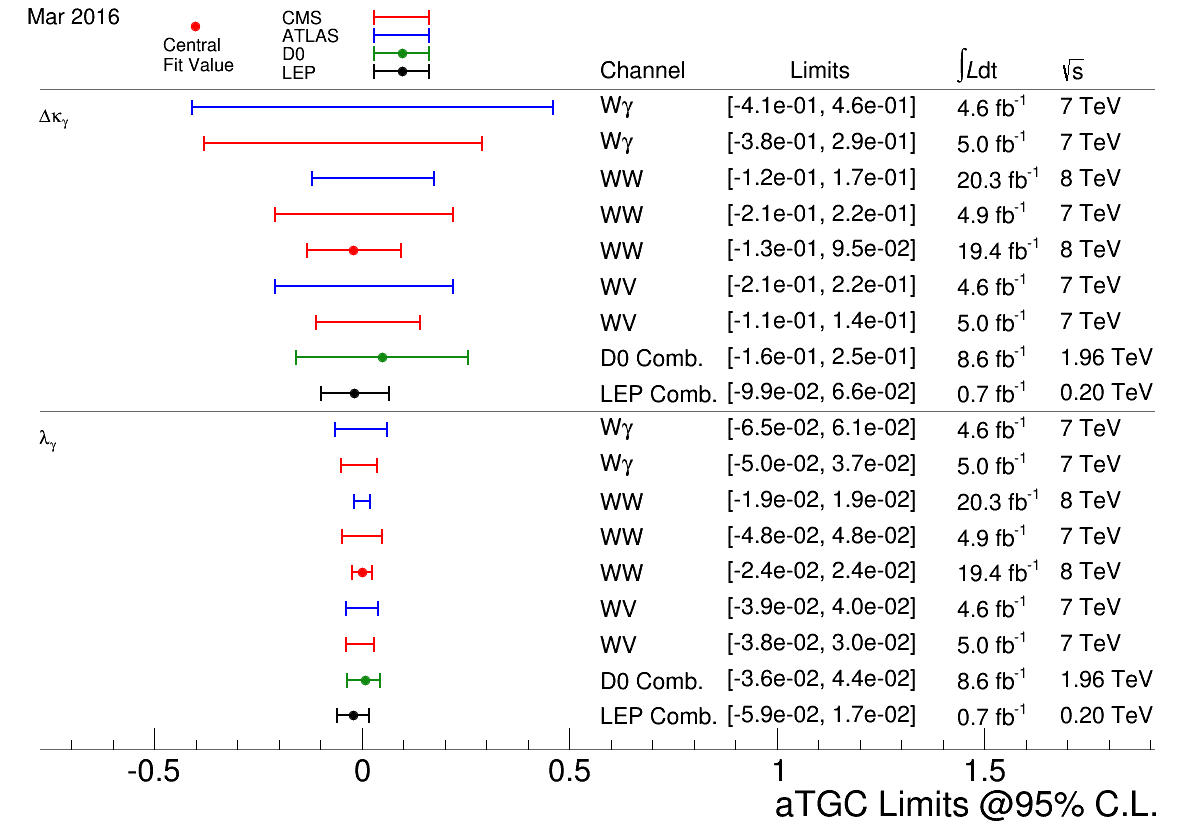
\includegraphics[width=0.80\textwidth]{../figs/WgAbout/aTGC_cg.png}}
    \caption{Summary of limits on the $WW\gamma$ aTGC coupling constants. Figure from~\cite{ref_twiki_SMP_ATGC}.}
    \label{fig:aTGC_cg}
  \end{center}
\end{figure}
The most recent measurements of $W\gamma$ production were performed by CMS~\cite{ref_7TeV_CMS} and ATLAS~\cite{ref_7TeV_ATLAS} collaborations with $pp$ collisions at $\sqrt{s}=7$~GeV collected in~2011. Both collaborations considered two channels: $W\gamma\rightarrow\mu\nu\gamma$ and $W\gamma\rightarrow e\nu\gamma$.\\
%The measurements are based on~5~fb$^{-1}$ and~4.6~fb$^{-1}$ of integrated luminosity with CMS and ATLAS respectively.
Diboson processes are rare in $pp$-collisions and analysts have to filter out events of their interest from many processes which are more likely to happen. To do that, a variety of selection criteria are applied which reject most of the background events to increase the signal fraction in the selected sample as much as possible. However, even after all possible selection criteria are applied, the majority of selected events are still background events and it is not possible to reduce the background any further without also significantly reducing signal.\\
The major source of such irreducible background is the fake photon background where hadronic jets are misidentified as photons. Such events originate mostly from $W+$jets, but $Z+$jets and $\bar{t}t+$jets events contribute to this source of background as well. In the electron channel there is one more significant background that is the fake photon background where electron is misidentified as a photon.  Such events are coming from $Z+$jets events. For the muon channels this background is small. Other sources of backgrounds for both channels include real-$\gamma$, fake lepton + real photon and fake lepton + fake photon backgrounds. The major source of real-$\gamma$ background is the $Z\gamma$ process where a final state lepton and a photon mimics the $W\gamma$ final state. Fake lepton + real photon background originates from the $\gamma+$jets process where a jet is misidentified as a lepton. Fake lepton + fake photon backgrounds come from dijet and multijet events where one of the jets is misidentified as a lepton and the other one is misidentified as a photon. The probability of a jet to be misidentified as a lepton is very small, therefore fake lepton + real photon and fake lepton + fake photon backgrounds are negligible.\\
$P_T^\gamma$ spectra are measured because this variable is the most sensitive to the potential aTGC. The $P_T^\gamma$ spectra of the selected events in data superimposed with selected events in the simulation of the signal and estimated background contribution for the muon and electron channels are shown in Fig.~\ref{fig:Wg7TeV_CMS_ptGamma} for CMS and in Fig.~\ref{fig:Wg7TeV_ATLAS_ptGamma} for ATLAS measurement. Both measurements show a good agreement between data and the simulation.\\
%To derive aTGC limits...
\begin{figure}[htb]
  \begin{center}
    {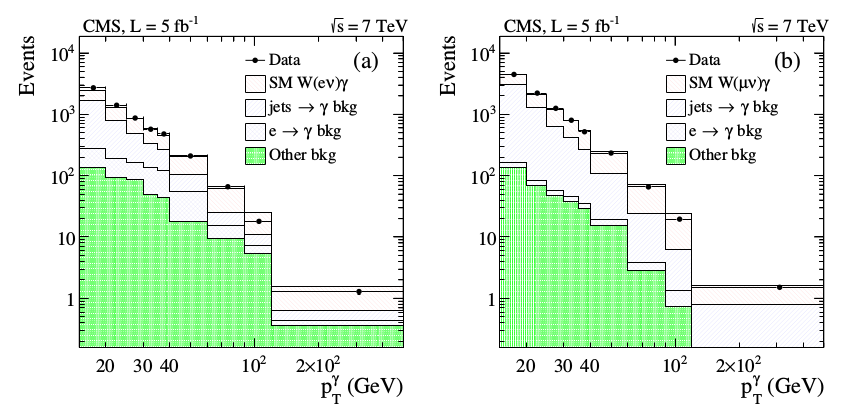
\includegraphics[width=0.80\textwidth]{../figs/WgAbout/Wg7TeV_CMS_ptGamma.png}}
    \caption{The distribution of the $p_T^\gamma$ of W$\gamma$ candidates in the analysis of~7~TeV CMS data. Data vs signal MC + background estimates. Left: $W\gamma\rightarrow e\nu\gamma$, right: $W\gamma\rightarrow \mu\nu\gamma$~\cite{ref_7TeV_CMS}.}
    \label{fig:Wg7TeV_CMS_ptGamma}
  \end{center}
\end{figure}
\begin{figure}[htb]
  \begin{center}
    {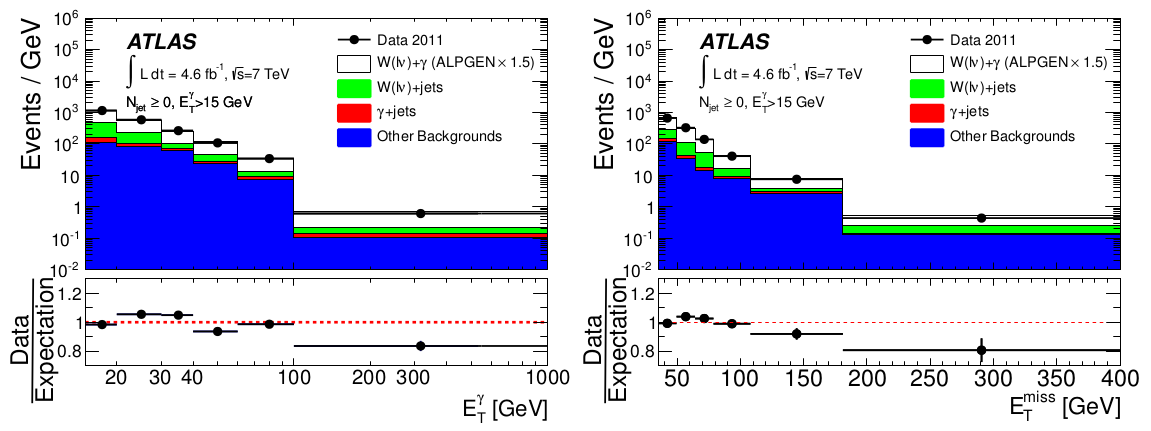
\includegraphics[width=0.80\textwidth]{../figs/WgAbout/Wg7TeV_ATLAS_ptGamma.png}}
    \caption{The distribution of the photon transverse momentum (left) and missing transverse momentum (right) of W$\gamma$ candidates in the analysis of 7 TeV ATLAS data. Data vs signal MC + background estimates~\cite{ref_7TeV_ATLAS}. }
    \label{fig:Wg7TeV_ATLAS_ptGamma}
  \end{center}
\end{figure}
The phase space restrictions of $W\gamma$ measurements come from the considerations of the detector acceptance, reducing heavily background-dominated regions and theoretical considerations such as to avoid divergence of the cross section and to reduce ISR and FSR contributions to the cross section.\\
CMS provides measurements of the $P_T^\gamma$ spectrum, the total cross section within the phase spaces of $\Delta R>0.7$, $P_T^\gamma>15$~GeV, $P_T^\gamma>60$~GeV and $P_T^\gamma>90$~GeV.\\
ATLAS, in addition to the $P_T^\gamma$ spectrum, total cross section and limits, provides the differential cross section and cross section with different number of associated jets. The phase space restrictions for ATLAS measurement include requirements on charged lepton kinematics $P_T^l>25$~GeV, $|\eta_l|<2.47$, requirements on the transverse momentum of a neutrino $P_T^\nu>35$~GeV, photon kinematics $P_T^\gamma>15$~GeV, $|\eta^\gamma|<2.37$, photon isolation fraction $\epsilon^P_h<0.5$ and lepton-photon separation $\Delta R(l,\gamma)>0.7$. For the differential cross section in number of associated jets, the requirements on jets kinematics and jets separation from leptons and photons are also applied: $E_T^{jet}>30$~GeV, $|\eta^{jet}|<4.4$, $\Delta R(e/\mu/\gamma,jet)>0.3$. No evidence of new physics is observed.\\
The estimated cross sections with any number of associated jets for $P_T^\gamma>15$~GeV are \\
\begin{equation}
\sigma(pp\rightarrow W\gamma\rightarrow l\nu\gamma) = 37.0 \pm 0.8\text{~(stat.)~}\pm 4.0\text{~(syst.)~}\pm 0.8\text{~(lumi.)~pb}
\end{equation}
\noindent{and} \\
\begin{equation}
\sigma(pp\rightarrow W\gamma\rightarrow l\nu\gamma) = 2.77 \pm 0.03\text{~(stat.)~}\pm 0.33\text{~(syst.)~}\pm 0.14\text{~(lumi.)~pb}
\end{equation}
\noindent{for CMS and ATLAS respectively. The results agree with NLO MCFM~\cite{ref_MCFM}  predictions of $31.81 \pm 1.8$~pb for the phase space used by CMS and of $1.96 \pm 0.17$~pb for the phase space used by ATLAS.}\\
In addition to the cross sections, both CMS and ATLAS provide limits on aTGC coupling constants $\Delta \kappa_\gamma$ and $\lambda_\gamma$. To do that, samples with non-zero aTGC coupling constants are generated, run through the whole reconstruction and selection procedures, and compared to the measured results of $P_T^\gamma$ spectra. The results on one-dimensional limits are quoted in Fig.~\ref{fig:aTGC_cg} while the results on two-dimensional limits can be found in~\cite{ref_7TeV_ATLAS},~\cite{ref_7TeV_CMS}.\\
In this dissertation we are measuring total and differential $d\sigma/d P_T^\gamma$ cross section. While the aTGC limits are not derived in this dissertation, the measured differential cross section can be used to derive them. The measurement details and results are described in Chapter~\ref{sec:AN_WgMeas}.\\
